\documentclass[a4paper,11pt]{article}

\usepackage{mlsubmit}

\begin{document}

\initmlsubmision{2}            	% assignment number
								{Abhisek Panda}  		% your name
								{150026}					% your roll number


%% -----------------Question 1-----------------------


\begin{mlsolution}

\subsection{subPart 1:}
Yes. Observe \\
entry 4(C. Binns, medium, no, heavy, 0-1, NO) and\\
entry 6(S. Snape, medium, no, heavy, 0-1, YES)\\
In these data points, the decisions are different even though all parameters except name of professor are identical. Hence, it must be the case that name of professor was the criteria to distinguish both data points.

\subsection{subPart 2:}
Yes, if there exists a novel algorithm to extract information from the names of the professors then its possible. Otherwise not. On a side note,

\subsection{subPart 3:}
\begin{align*}
Entropy(S)  &= -\frac{5}{15} \log\frac{5}{15} - \frac{10}{15} \log\frac{10}{15}\\
			&= 0.9183
\end{align*}
Information Gain for each attribute is calculated as:
$$ Gain(S, A) = Entropy(S) - \Sigma_{v} \frac{|S_v|}{|S|} Entropy(S_v)$$
where $S_v$ is the subset of S where attribute A gets value v.
%\begin{align*}
%	Entropy(S_{size=small}) &= -\frac{1}{6} \log\frac{1}{6} - \frac{5}{6} \log\frac{5}{6}\\
%							&= 0.6500\\
%	Entropy(S_{size=medium}) &= -\frac{2}{5} \log\frac{2}{5} - \frac{3}{5} \log\frac{3}{5}\\
%							&= 0.9710\\
%	Entropy(S_{size=large}) &= -\frac{2}{4} \log\frac{2}{4} - \frac{2}{4} \log\frac{2}{4}\\
%							&= 1.0\\
%	Entropy(S_{like=yes})	&= -\frac{2}{4} \log\frac{2}{4} - \frac{2}{4} \log\frac{2}{4}\\
%							&= 1.0\\ 
%	Entropy(S_{like=no})	&= -\frac{3}{11} \log\frac{3}{11} - \frac{8}{11} \log\frac{8}{11}\\
%							&= 0.8454\\ 
%	Entropy(S_{workload=light})	&= -\frac{1}{4} \log\frac{1}{4} - \frac{3}{4} \log\frac{3}{4}\\
%							&= 0.8113\\
%	Entropy(S_{workload=average}) &= -\frac{3}{6} \log\frac{3}{6}-\frac{3}{6} \log\frac{3}{6}\\
%							&= 1.0\\ 
%	Entropy(S_{workload=heavy})	&= -\frac{1}{5} \log\frac{1}{5} - \frac{4}{5} \log\frac{4}{5}\\
%							&= 0.7219\\
%	Entropy(S_{\#meetings=0-1})	&= -\frac{4}{10} \log\frac{4}{10} - \frac{6}{10} \log\frac{6}{10}\\
%							&= 0.9710\\ 
%	Entropy(S_{\#meetings=2-3})	&= -\frac{0}{3} \log\frac{0}{3} - \frac{3}{3} \log\frac{3}{3}\\
%							&= 0\\
%	Entropy(S_{\#meetings>3})	&= -\frac{0}{2} \log\frac{0}{2} - \frac{2}{2} \log\frac{2}{2}\\
%							&= 0\\ 
%\end{align*}
%The last 2 entropies follow from the fact that $\underset{x \rightarrow 0}{\lim}\ x\log x = 0$.

Therefore,
\begin{align*}
	Gain(S, size) &= 0.9183 - \frac{6}{15}0.6500 - \frac{5}{15}0.9710 - \frac{4}{15}1\\
					&= 0.0680\\
	Gain(S, like) &= 0.9183 - \frac{4}{15}1 - \frac{11}{15}0.8454\\
					&= 0.0317\\
	Gain(S, workload) &= 0.9183 - \frac{4}{15}0.8113 - \frac{6}{15}1.0 - \frac{5}{15}0.7219\\
					&= 0.0613\\
	Gain(S, \#meetings) &= 0.9183 - \frac{10}{15}0.9710 - \frac{3}{15}0 - \frac{2}{15}0\\
					&= 0.2710 \\
\end{align*}

Hence, the decision tree should have Number of Meetings as its root since it gives us the highest information gain. For further splitting,
\begin{align*}
	Gain(S_{0-1}, workload) &= 0.9710 - \frac{2}{10}1 - \frac{3}{10}0 - \frac{5}{10}0.7219\\
	&= 0.4100\\
	Gain(S_{0-1}, research\ area) &= 0.9710 - \frac{3}{10}0.9183 - \frac{7}{10}0.9852\\
	&= 0.0587\\
	Gain(S_{0-1}, size) &= 0.9710 - \frac{1}{10}0 - \frac{5}{10}0.9710 \frac{4}{10}1\\
		&= 0.085
\end{align*}
So the next node is workload. After this level, nodes can be split on the basis of majority.
\begin{figure}[th]%
	\centering
	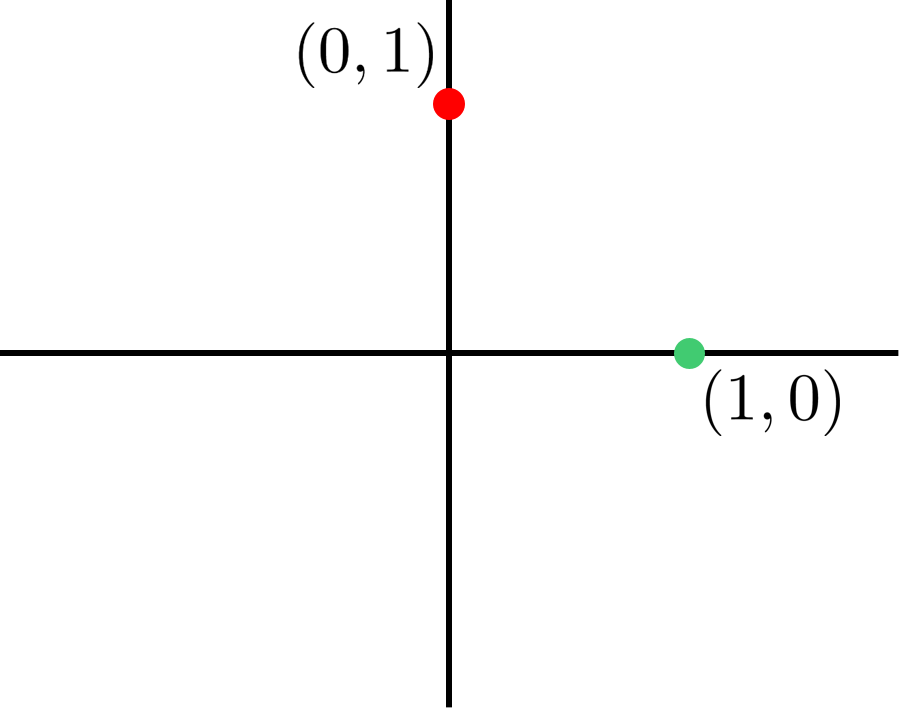
\includegraphics[width=0.5\columnwidth]{proto_blank.png}%
	\hfill
	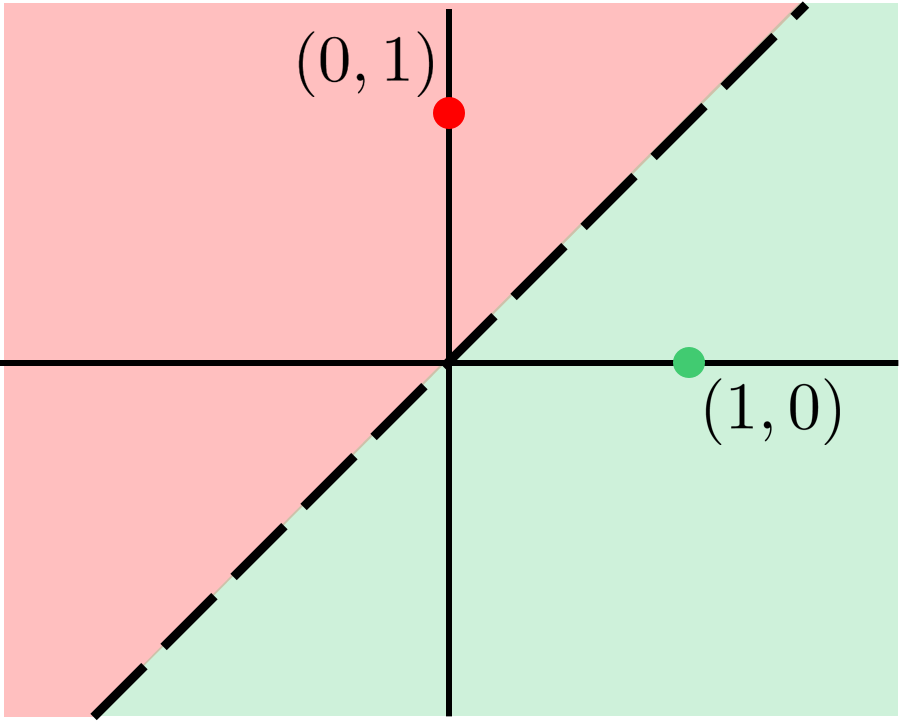
\includegraphics[width=0.5\columnwidth]{proto_euclid_sample.png}%
	\caption{Learning with Prototypes: the figure on the left shows the two prototypes. The figure on the right shows what the decision boundary if the distance measure used is $d(\vz^1,\vz^2) = \norm{\vz^1-\vz^2}_2$, for any two points $\vz^1,\vz^2 \in \bR^2$. The decision boundary in this case is the line $y = x$.}%
	\label{fig:proto}%
\end{figure}
\end{mlsolution}


%% -----------------Question 2-----------------------


\begin{mlsolution}
	\subsection{subPart1:}
	The products purchased by a customer is represented by a L dimensional vector $\vS$ where $\vS_j = 1$ implies customer purchased that product. Otherwise, it is 0.
	To model $\P{b\cond\vx,\vTheta}$ where $b$ is the bill of the items purchased by the customer $\vx$.
	\begin{align*}
		\P{b\cond\ \vx, \vTheta} &= \sum_{i=1}^{2^L} \P{b\cond\ \vx, \vS^i, \vTheta} \P{\vS^i\cond\ \vx, \vTheta}
	\end{align*}
	Since the bills have an added gaussian noise, the conditional probability $$\P{b\cond\ \vx, S^i, \vTheta} = \mathcal{N}(\mu_i, \sigma^2)$$
	Also, assuming the choice between various products as independent when conditioned with the customers, $\P{\vS^i\cond\ \vx, \vTheta} = \prod_{j=1}^{L} \P{\vS^i_j\cond\ \vx, \vTheta}$.\\
	Assume $\P{\vS^i_j=1\cond\ \vx, \vTheta} = \sigma(w_j^T\vx^i)$ where $\sigma$ is the sigmoid function.\\
	The model for a single customer is given as:
	$$P[b^i \cond \vx^i, \vTheta] = \sum_{j=1}^{2^L} \P{b^i\cond\ \vx^i, \vS^j, \vTheta} * \left[\prod_{k=1}^{L} \P{\vS^j_k\cond\ \vx^i, \vTheta}\right]$$
	Thus, the latent variables are the purchased items vectors, $S^i$s.
	The model $\vTheta$ consists of weight vectors $w_j$ for each product($j \in [L]$),  $\mu_i$ for each customer and a $\sigma$ which is same noise for every customer.
	
	\subsection{subPart 2:}
	The likelihood expression for the above objective function is obtained by multiplying the probabilities for each customer:
	\begin{align*}
	P[\vb\ \cond \vX, \vTheta] &= \prod_{i=1}^{n} P[b^i \cond \vx^i, \vTheta]\\
	P[\vb\ \cond \vX, \vTheta] &= \prod_{i=1}^{n}\sum_{j=1}^{2^L} \P{b^i\cond\ \vx^i, S^j, \vTheta} * \left[\prod_{k=1}^{L} \P{S^j_k\cond\ \vx^i, \vTheta}\right]\\
	&= \prod_{i=1}^{n}\sum_{j=1}^{2^L} \cN\left(\mu_j,\sigma^2\right) * \left[\prod_{k=1}^{L} \P{S^j_k\cond\ \vx^i, \vTheta}\right]	\\
	\implies \vTheta_{MLE}& = \underset{\vTheta}{\arg\max}\ P[\vb\cond \vX, \vTheta]
	\end{align*}
	
	
	\subsection{subPart 3:}
	Hard Assignment Alternating Optimization:\\
	\begin{enumerate}
		\item Initialize $\vTheta^0$.
		\item For $i \in [n]$, update $S^i$. This can be done by choosing $S^i$ such that the probability $P[S\cond \vx^i, b^i, \vTheta^t]$ is maximum.
			\begin{align*}
				S^i &=  \underset{S}{\arg\max}\ P[S\cond\ \vx^i, b^i, \vTheta] \intertext{where}
				\P{S\cond\ \vx^i, b^i, \vTheta}
							&\propto P[S \cond \vx^i, \vTheta]\ P[b^i\cond x^i, S, \vTheta]\\
							&= \mathcal{N}(\mu^i, \Sigma)\prod_{j=1}^{L} \P{S_j\cond\ \vx^i, b^i, \vTheta}\\
							&= \mathcal{N}(\mu^i, \Sigma)\prod_{j=1}^{L} \sigma(\vw_j^T\vx^i)^{S_j} * [1 - \sigma(\vw_j^T\vx^i)]^{1 - S_j}
							\intertext{Hence, this reduces to setting all the $S_j^i$ as 1 or 0 depending on whose probabilty is greater than $0.5$}
			\end{align*}
		\item Update $\vTheta^{t+1}$ using the new obtained $S^i$.
			\begin{align*}
				\vTheta^{t+1} &= \underset{\vTheta}{\arg \max} P[B, S | X, \vTheta]\\
							&= \underset{\vTheta}{\arg \max} \prod_{i=1}^{n} P[b^i \cond S^i, x^i, \vTheta]\ P[S^i \cond x^i, \vTheta]\\
							&= \underset{\vTheta}{\arg \max} \prod_{i=1}^{n} \mathcal{N}(\mu^i, \sigma^2)
							\prod_{j=1}^{L}P[S^i_j\cond \vx^i, \vTheta]\\
							&= \underset{\vTheta}{\arg \max} \prod_{i=1}^{n} \left(\mathcal{N}(\mu^i, \sigma^2)
							\prod_{j=1}^{L}\sigma(\vw_j^T\vx^i)^{S_j^i} * [1 - \sigma(\vw_j^T\vx^i)]^{1 - S_j^i}\right)
							\intertext{Taking log and solving for MLE(using first order derrivative for $\mu$ and $\sigma$) for this objective function; we get:}
							\mu_i &= \sum_{j|S^i_j = 1} C_j\\
							\sigma_i^2 &=  \frac{\sum_{i=1}^{n}(x^i - \mu^i)^2}{n}
							\intertext{The $\vw_j$s can be obtained by performing logistic regression in $O(nd)$ time.}
			\end{align*}
	\end{enumerate}
	\newpage
	\subsection{subPart4:}
	The soft Alternating optimization algorithm is as follows:
	\begin{enumerate}
		\item For $i \in [n]$ create $2^L$ copies of datapoint $x^i$.
			\begin{itemize}
				\item Let $x^i \rightarrow \{x^{i,1}, x^{i,2},..., x^{i,2^L}\}$
			\end{itemize}
		\item Initialize $\vTheta^0$.
		\item Update weights $\gamma^{i,k,t}$ using $\vTheta^0$
				\begin{align*}
					\gamma^{i,k,t} &= P[S^i | b^i, \vx^i, \vTheta^t]\\
					&= \frac{P[S^i = k \cond \vx^i, \vTheta]\ P[b^i\cond x^i, S^i = k, \vTheta]}
					{\sum_{j=1}^{j=2^L}P[S^i = j\cond \vx^i, \vTheta]\ P[b^i\cond x^i, S^i = j, \vTheta]}\\
					&= \frac{\mathcal{\vpi}_k^t\ \mathcal{N}(\mu_i, \sigma^2)}
					{\sum_{j=1}^{j=2^L}\mathcal{\vpi}_j^t\ \mathcal{N}(\mu_i, \sigma^2)}
				\end{align*}
				where $\mathcal{\pi}_k = P[S^i = k | \vx^i, \vTheta]$ which is the product of linear logistic models as described previously.
		\item Update $\vTheta^{t+1}$,
		\begin{align*}
			\vTheta^{t+1} &= \underset{\vTheta}{\arg\max}\ P[\{\vx^{i,k}\}, \{b^{i,k}\}, \{\gamma^{i,k,t}\}]
		\end{align*}
		where $P[\vx,b,\gamma\ |\vTheta] = P[x,b|\vTheta]^\gamma$.
	\end{enumerate}
	
	
	
\end{mlsolution}


%% -----------------Question 3-----------------------


\begin{mlsolution}
	Given objective function is:
\begin{align*}
\underset{\vw,\bc{\xi_i}}{\arg\min}&\ \norm{\vw}_2^2 + \sum_{i=1}^n\xi_i^2\\
\text{s.t.} &\ y^i\ip{\vw}{\vx^i} \geq 1 - \xi_i, \text{ for all } i \in [n] \qquad\qquad(P1)\\
&\ \xi_i \geq 0, \text{ for all } i \in [n]
\end{align*}

\subsection{subPart1:}
To show that $\xi_i \geq 0$ are vacuous. Let $\xi_i$ be negative, if possible, in the optimal solution obtained with corresponding objective value $H$. Observe the constraint $y^i\ip{\vw}{\vx^i} \geq 1 - \xi_i$. Since $\xi_i$ is negative; $1 - \xi_i > 1 - 0 \implies y^i\ip{\vw}{\vx^i} > 1\ (-0) $. Hence, we can always replace a negative $\xi_i$(if obtained) with a 0. Clearly, this reduces the objective function value to $H^{\prime}$, since $\xi_i^2 \geq 0\ \forall i$. This leads to a contradiction since we had assumed that the original H is the optimal value.
\subsection{subPart2:}
\begin{align*}
	y^i\ip{\vw}{\vx^i} &\geq 1 - \xi_i\\
	\implies 1 - \xi_i - y^i\ip{\vw}{\vx^i} &\leq 0\\
	\intertext{and the constraint for $\xi_i$}
	\xi_i &\geq 0\\
	\implies -\xi_i &\leq 0
\end{align*}
% So, introduce parameters $\alpha_i$ so that the langrangian becomes:
So, introduce parameters $\alpha_i$ and $\beta_i$  so that the langrangian becomes:
% $$ L(\vw,\bc{\xi_i}, \bc{\alpha_i}) = \norm{\vw}_2^2 + \sum_{i=1}^n\xi_i^2 + \sum_{i=1}^n \alpha_i(1 - \xi_i - y^i\ip{\vw}{\vx^i}) \qquad\qquad(L1)$$
$$ L(\vw,\bc{\xi_i}, \bc{\alpha_i}, \bc{\beta_i}) = \norm{\vw}_2^2 + \sum_{i=1}^n\xi_i^2 + \sum_{i=1}^n \alpha_i(1 - \xi_i - y^i\ip{\vw}{\vx^i}) - \sum_{i=1}^{n}\beta_i\xi_i \qquad\qquad(L1)$$
					
\subsection{subPart3:}
The objective is to solve $$\underset{\vw,\bc{\xi_i}}{\arg\min}\ \underset{\alpha_i \geq 0, \beta_i \geq 0}{\arg\max}\ \ L(\vw,\bc{\xi_i}, \bc{\alpha_i}, \bc{\beta_i})$$
Taking derrivative w.r.t $\vw$, we get:
\begin{align*}
	0 &= 2\vw + 0 + \sum_{i=1}^{n} \alpha_i * (-y^i\vx^i)\\
	\implies \vw &= \frac{\sum_{i=1}^{n} \alpha_iy^i\vx^i}{2}
\end{align*}
Similarly, taking derrivative w.r.t $\xi_i$, we get:
\begin{align*}
	0 &= 2\xi_i - \alpha_i - \beta_i
	\implies \xi_i = \frac{\alpha_i + \beta_i}{2}
\end{align*}
Substituting these values in equation (L1), we get:
\begin{align*}
	f(\bc{\alpha_i}, \bc{\beta_i}) 
			&= \frac{1}{4}\sum_{i=1}^{n}\sum_{j=1}^{n}\alpha_i\alpha_jy^iy^j(\vx^i)^T\vx^j + \frac{1}{4}\sum_{i=1}^{n}(\alpha_i +\beta_i)^2 +
			\sum_{i=1}^n\alpha_i
			- \sum_{i=1}^n \alpha_i y^i \ip{\frac{1}{2}\sum_{j=1}^{n} \alpha_j y^j \vx^j}{\vx^i}\\
			& \qquad\qquad-\frac{1}{2}\alpha_i(\alpha_i + \beta_i) -\frac{1}{2}\beta_i(\alpha_ + \beta_i)\\
			&= \sum_{i=1}^n \alpha_i -\frac{1}{4}\sum_{i=1}^{n}\sum_{j=1}^{n}\alpha_i\alpha_jy^iy^j(\vx^i)^T\vx^j - \sum_{i=1}^n\frac{(\alpha_i + \beta_i)^2}{4}
\end{align*}
which is the required answer.

\subsection{subPart 4:}
Dual Problem for (P1) is given by: $$f(\bc{\alpha_i}, \bc{\beta_i}) = \sum_{i=1}^n \alpha_i - \sum_{i=1}^n\frac{(\alpha_i + \beta_i)^2}{4} - \frac{1}{4} \sum_{i=1}^{n}\sum_{j=1}^{n}\alpha_i\alpha_jy^iy^j(\vx^i)^T\vx^j$$ subject to the constraints: $\alpha_i \geq 0, \beta_i \geq 0$.\\
Note that the dual objective is maximized when $(\alpha_i + \beta_i)^2$ is as small as possible. Since $\beta$ only appears in this term, we can conveniently set it to 0($\beta_i \geq 0$). This implies that the original constraint of $\xi_i \geq 0$ was vacuous since it does not contribute to finding the optima.\\
Hence, the new Dual Problem becomes:
$$ f(\bc{\alpha_i}) = \sum_{i=1}^n \alpha_i - \sum_{i=1}^n\frac{\alpha_i^2}{4} - \frac{1}{4} \sum_{i=1}^{n}\sum_{j=1}^{n}\alpha_i\alpha_jy^iy^j(\vx^i)^T\vx^j$$ subject to the constraints: $\alpha_i \geq 0$ 
\\ \\ 
Dual problem for original SVM is given by:
$$f(\alpha) = \sum_{i=1}^n \alpha_i - \frac{1}{2} \sum_{i=1}^{n}\sum_{j=1}^{n}\alpha_i\alpha_jy^iy^j(\vx^i)^T\vx^j$$
subject to the constraints: $0 \leq \alpha_i \leq C$

Clearly, there is an extra term in order of $ \sum_{i=1}^n \alpha_i^2$ due to taking $\xi_i^2$ instead of $\xi_i$ in (P1). Moreover, there is an additional upper bound on $\alpha_i$ in the original SVM dual problem, which is due to the extra requirement of $\xi_i \geq 0$ there. No such constraint is to be satisfied in dual for (P1) as proved in subPart(1).


\end{mlsolution}

%% -----------------Question 4-----------------------


					
\end{document}